%%%%%%%%%%%%%%%%%%%%%%%%%%%%%%%%%%%%%%%%%%%%%%%%%%%%%%%%%%%%%
%% Thyristor-based rectifiers %%
%%%%%%%%%%%%%%%%%%%%%%%%%%%%%%%%%%%%%%%%%%%%%%%%%%%%%%%%%%%%%
\section{Thyristor-based rectifiers}

%%%%%%%%%%%%%%%%%%%%%%%%%%%%%%%%%%%%%%%%%%%%%%%%%%%%%%%%%%%%%
%% Thyristor: an externally switchable power electronic component %%
%%%%%%%%%%%%%%%%%%%%%%%%%%%%%%%%%%%%%%%%%%%%%%%%%%%%%%%%%%%%%
\begin{frame}[c]
    \frametitle{Thyristor: an externally switchable power electronic component}
    \begin{columns}
        \begin{column}{0.66\textwidth}
            \begin{itemize}
                \item Can block voltage in both directions (when off)
                \begin{itemize}
                    \item Different to diode (only blocks reverse voltage)
                \end{itemize}
                \item Can conduct current in only one direction (when on)
                \begin{itemize}
                    \item Identical to diode
                \end{itemize}
                \item Turn-on: via gate signal
                \item Turn off: via current drop below holding current \\(i.e., depends on load characteristics and input voltage)
            \end{itemize}
            \vspace{-0.7cm}
            \begin{varblock}{Application area}
                While transistors are used for high-frequency converters due to their favorable turn-on/off characteristics and have replaced thyristors in many cases, the latter are still used in low switching frequency applications (mostly energy grid) due to their favorable high voltage / current ratings. 
            \end{varblock}
        \end{column}
        \begin{column}{0.33\textwidth}
                \centering
        
                \begin{circuitikz}
                    \draw (0,0) to [thyristor, v=$u$, i=$i$, voltage = straight, name = T] (2,0);
                    \node at (T.gate) [above]{\footnotesize\hl{Gate}};
                    \node at (0,0) [left]{\footnotesize\hl{Anode}};
                    \node at (2,0) [right]{\footnotesize\hl{Cathode}};
                \end{circuitikz}\\[2em]

                \begin{figure}
                    \begin{tikzpicture} 
                        \hphantom{$s$}
                        \begin{axis}[
                            xmin=-1, xmax=1,
                            ymin=-1, ymax=1,
                            width=0.8\textwidth,
                            height=0.5\textheight,
                            axis lines=middle,
                            clip = false,
                            thick,
                            xlabel = {$u$},
                            ylabel = {$i$},
                            xticklabels=\empty,
                            xlabel style={anchor = west},
                            ylabel style={anchor = north east},
                            yticklabels=\empty,
                            anchor = center
                            ]
                            \addplot[signalred, very thick] coordinates {(-1,0) (1,0)};
                            \addplot[signalgreen, very thick] coordinates {(0,0) (0,1)};
                            \draw [pin] (axis cs:-0.05,0.5) -- +(-10pt,-5pt) node[left, align=center, font=\footnotesize ] {active\\ gate};
                            \draw [pin] (axis cs:0.05,0.5) -- +(10pt,-5pt) node[right, align=center, font=\footnotesize ] {no turn\\off};
                            \draw [pin] (axis cs:0.25,-0.05) -- +(12pt,-10pt) node[below, align=center, font=\footnotesize ] {disabled\\ gate};
                        \end{axis}
                    \end{tikzpicture}
                    \caption{Idealized thyristor characteristics and circuit symbol}
                    \label{fig:thyristor}
                \end{figure}
        \end{column}
    \end{columns}
\end{frame}

%%%%%%%%%%%%%%%%%%%%%%%%%%%%%%%%%%%%%%%%%%%%%%%%%%%%%%%%%%%%%
%% Thyristor examples %%
%%%%%%%%%%%%%%%%%%%%%%%%%%%%%%%%%%%%%%%%%%%%%%%%%%%%%%%%%%%%%
\begin{frame}[b]
    \frametitle{Thyristor examples}
    \begin{figure}
        \begin{subfigure}{0.45\textwidth}
            \centering
			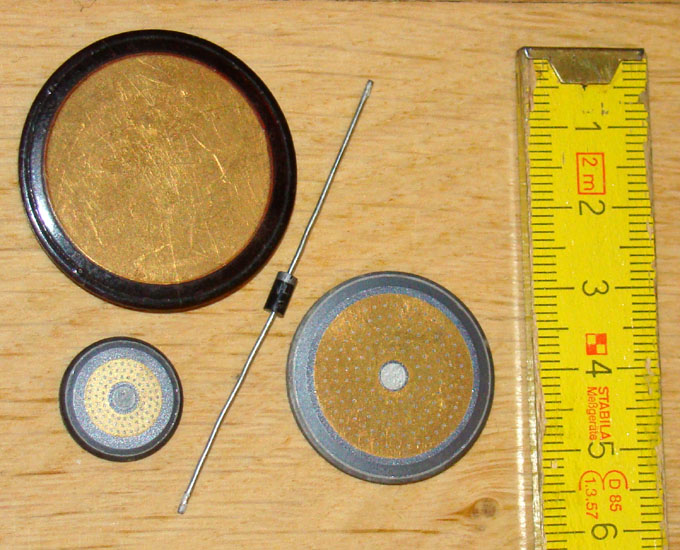
\includegraphics[height=0.45\textheight]{fig/lec05/Thyristor_example_01.jpg}
			\caption{top left: \SI{1000}{\volt}/\SI{200}{\ampere}; bottom left: \SI{1500}{\volt}/\SI{20}{\ampere}; right: \SI{1500}{\volt}/\SI{120}{\ampere}; 1N4007 diode for comparison (source: \href{https://de.wikipedia.org/wiki/Datei:SCR_power_rectifiers.jpg}{Wikimedia Commons}, \href{https://creativecommons.org/publicdomain/zero/1.0/}{CC0~1.0})}
        \end{subfigure}
        \hspace{1cm}
        \begin{subfigure}{0.45\textwidth}
            \centering
            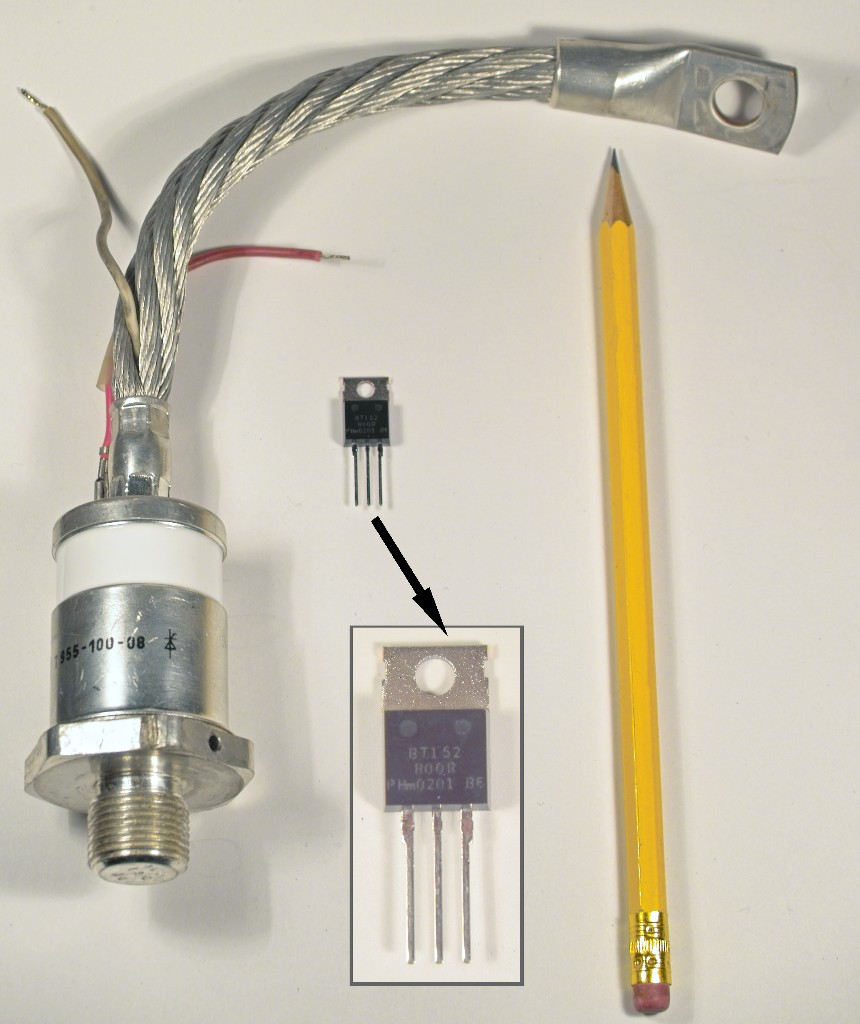
\includegraphics[height=0.45\textheight]{fig/lec05/Thyristor_example_02.jpg}
			\caption{left: \SI{800}{\volt}/\SI{100}{\ampere}; right: \SI{800}{\volt}/\SI{13}{\ampere} (source: \href{https://de.wikipedia.org/wiki/Datei:Thyristors_thyristoren.jpg}{Wikimedia Commons}, Julo, \href{https://creativecommons.org/licenses/by-sa/3.0/deed.de}{CC0~BY-SA~3.0})}
            \vspace{2em}
        \end{subfigure}
        \caption{Thyristor examples with different voltage and current ratings}
        \label{fig:thyristor_examples}
    \end{figure}
\end{frame}

%%%%%%%%%%%%%%%%%%%%%%%%%%%%%%%%%%%%%%%%%%%%%%%%%%%%%%%%%%%%%
%% M1 rectifier comparison %%
%%%%%%%%%%%%%%%%%%%%%%%%%%%%%%%%%%%%%%%%%%%%%%%%%%%%%%%%%%%%%
\begin{frame}
    \frametitle{M1 rectifier comparison}

\end{frame}